\subsection{The ground states of the Rindler wedges \checkmark (bis auf Fragen)}
	But instead of integrating from $t_E= -\infty$ to 0, we choose the range of $\pi$ like in \textbf{Figure~\ref{eucpath}}. In addition our Hilbert space is separated in to $\Hil_L$ and $\Hil_R$ with the fields $\phi_L$ and $\phi_R$ so we write 
	\begin{align} \label{pathint}
		\braket{\phi_L \phi_R | \Omega} \propto \braket{\phi_R| e^{-\pi K_R} \Theta| \phi_L}_L
	\end{align}
	Here the $K_R$ is the operator $K_x$ but in the right Rindler wedge while the operator $\Theta$ which is antiunitary\footnote{unitary would mean for a linear operator $A$: $A^\dagger A = \mathds{1}$ so $\braket{Ax|Ay}=\braket{x|y}$, antiunitary would be a antilinear operator $A$ ($\braket{x|A^\dagger}=\braket{y|Ax}$) which also fulfills: $\braket{Ax|Ay}=\braket{y|x}$. },also called CPT and exists in all quantum field theories. It acts on a scalar field in the Heisenberg picture like $\Theta^\dagger \phi(t,x,y,z)\Theta = \phi^\dagger(-t,-x,y,z)$ which gives a map between the to Hilbert spaces. This is important in \eqref{pathint} because \marginpar{warum e hoch -pi, was ist das i in der summe, was ist omega i und v.a. warum steht manchmal ein L oder ein R außerhalb der Kets}
		\begin{enumerate}
			\item $\braket{\phi_L \phi_R| \Omega}$ can now be described just with a matrix in $\Hil_R$
			\item the $\phi_L$ is playing the role of a final state, the $\phi_R$ the role of the initial state in \textbf{Figure \ref{eucpath}}.
		\end{enumerate}
	Now we can evaluate \eqref{eucpath}:
	\begin{align}
		\braket{\phi|\Omega} &\propto \sum_i e^{-\pi \omega_i} \braket{i | \Theta | \phi_L} \braket{\phi_R|i}_R \nonumber\\
		&\propto \sum_i e^{-\pi \omega_i} \braket{\phi_L| i^*}_L\braket{\phi_R|i}_R
	\end{align} %nachrechnen
	We inserted a complete set of  $K_R$ eigenstates, used that $\Theta$ is antiunitary and defined: $\ket{i^*}_L = \Theta^\dagger \ket{i}_R$, so now the ground state is:
	\begin{align} \label{groundstate}
		\ket{\Omega} = \frac{1}{\sqrt{Z}} \sum_i  e^{-\pi \omega_i} \ket{i^*}_L \ket{i}_R 
	\end{align}
	In this connection Z is the partition function, a constant which is given through the normalization condition\footnote{The sum over all probabilities is equal to one. see p.11 \cite{Brenig}}. 
	
	Or we compute the density matrix of the right Rindler wedge (because see above: we just need the matrix of $\Hil_R$)
	\begin{align}
		\rho_R= \frac{1}{Z} \sum_i e^{-2\pi\omega_i} \ket{i}_R \bra{i}
	\end{align}
	which is the thermal density matrix with temperature $T=\frac{1}{2\pi}$. 
	\marginpar{warum T dimensionslos?}
	\begin{figure}[tbp]
		\begin{center}
			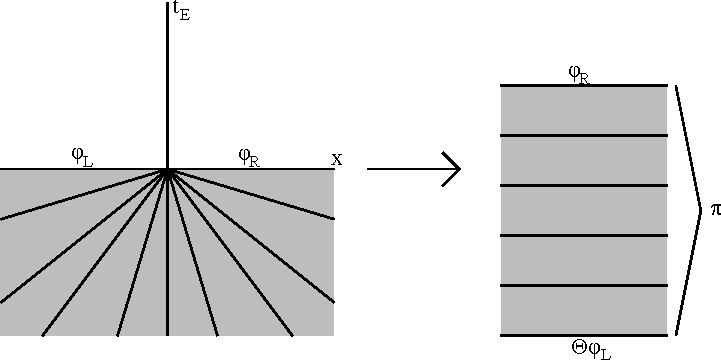
\includegraphics[scale=1]{eucpath}
			\caption{This is the Euclidean path integral representation changing \eqref{groundstate_phi} into a calculable integral, after we choose to integrate over an angle $\pi$. Note that $\varphi_R$ and $\varphi_L$ are the $\phi$s in the text.}\label{eucpath}
		\end{center}
	\end{figure}